\chapter{Correlation and Regression}

Correlation and regression are statistical methods that examine the relationship between two quantitative variables.

Correlation is concerned with quantifying the (linear) \emph{relationship} between two variables. Informally, it allows us to tell how strongly two variables move with each other. For instance, suppose we measure the heights and weights of a group of people. Intuitively, we would expect taller people to be heavier, hence there is a positive correlation between height and weight.

Regression, on the other hand, is concerned with quantifying how a change in one variable will affect the other variable. That is, regression predicts the value of a variable based on the value of the other variable. Reusing our previous example, regression allows us to predict the height of a person that weighs 70 kg.

\section{Independent and Dependent Variables}

When performing correlation and regression analysis, we need two sets of data, one for each variable. The resulting data is called bivariate data. A set of $n$ bivariate data can be expressed using ordered pairs $(x_i, y_i)$, where $x$ and $y$ are the two variables.

\begin{definition}
    In a bivariate relationship, the \vocab{independent variable} is the one that does not rely on changes in another variable, while the \vocab{dependent variable} is the one that depends on or changes in response to the independent variable.
\end{definition}

Informally, the independent variable is the variable we can ``control'' in an experiment, allowing us to vary its value to observe the resulting change in the value of the dependent variable.

\begin{recipe}
    To determine if there exists an independent/dependent relationship between two variables $x$ and $y$, we look at
    \begin{itemize}
        \item The context of the question -- Does one variable depend on the other?
        \item Key phrases in the question, e.g. ``investigate how $A$ depends on $B$'' means that $B$ is likely the independent variable and $A$ the dependent variable.
        \item Fixed or controlled variable in an experiment -- If a variable is manipulated in fixed increments, it is likely to be independent variable.
    \end{itemize}
\end{recipe}

Note however, that not all bivariate relationships have an independent and dependent variable. For instance, consider the following example:

\begin{example}
    Six newly-born babies were randomly selected. Their head circumference $x$ cm, and body length, $y$ cm were measured by the paediatrician and tabulated.

    \begin{table}[H]
        \centering
        \begin{tabular}{|c|c|c|c|c|c|c|}
        \hline
        $x$ & 31 & 32 & 33.5 & 34 & 35.5 & 36 \\ \hline
        $y$ & 45 & 49 & 47 & 50 & 53 & 51 \\ \hline
        \end{tabular}
    \end{table}

    All three heuristics for determining the independent/dependent relationship between $x$ and $y$ are not applicable. Hence, we say there is no clear independent and dependent variables, and we assume that no such relationship exists between the two variables.
\end{example}

\section{Scatter Diagram}

A scatter diagram is obtained when each pair of data value $(x_i, y_i)$ from a set of bivariate sample $\bc{(x_1, y_1), \dots, (x_n, y_n)}$ is plotted as a point on an $x$-$y$ graph.

\begin{recipe}[Drawing a Scatter Diagram]
    When drawing a scatter diagram, note that
    \begin{itemize}
        \item data points should be marked with a cross ($\times$);
        \item axes need not start from 0;
        \item axes need to be labelled according to context;
        \item the range of data values and the relative scale of the axes need to be indicated;
        \item the relative position of the points should be accurate.
    \end{itemize}
\end{recipe}

\begin{example}
    The number of employees, $y$, who stay back and continue in the office $t$ minutes after 5 pm on a particular day in a company is recorded. The results are shown in the table.

    \begin{table}[H]
        \centering
        \begin{tabular}{|c|c|c|c|c|c|c|c|}
        \hline
        $t$ & 15 & 30 & 45 & 60 & 75 & 90 & 105 \\ \hline
        $y$ & 30 & 19 & 15 & 13 & 12 & 11 & 10 \\ \hline
        \end{tabular}
    \end{table}

    Plotting the above points, we get our scatter diagram:
    \begin{figure}[H]\tikzsetnextfilename{477}
        \centering
        \begin{tikzpicture}[trim axis left, trim axis right]
            \begin{axis}[
                xlabel = {$t$},
                ylabel = {$y$},
                xtick = {15, 105},
                ytick = {30, 10},
                ylabel style={rotate=-90},
            ]
            \addplot [
                scatter,
                only marks,
                point meta=explicit symbolic,
                scatter/classes={
                    a={mark=x}
                },
            ] table [meta=label] {
                x    y   label
                15   30  a
                30   19  a
                45   15  a
                60   13  a
                75   12  a
                90   11  a
                105  10  a
            };
            \end{axis}
        \end{tikzpicture} 
        \caption{}
    \end{figure}
\end{example}

\subsection{Interpreting Scatter Diagrams}

There are four main relationships we can observe on a scatter diagram:
\begin{itemize}
    \item Positive linear relationship -- As $x$ increases, $y$ increases.
    \item Negative linear relationship -- As $x$ increases, $y$ decreases.
    \item Curvilinear relationship -- The points seem to lie on a curve.
    \item No clear relationship -- The points seem to be randomly scattered.
\end{itemize}

\begin{minipage}{0.5 \textwidth}
    \begin{figure}[H]\tikzsetnextfilename{478}
    \centering
    \begin{tikzpicture}[trim axis left, scale=0.8]
        \begin{axis}[
            xlabel = {$x$},
            ylabel = {$y$},
            xtick = {0, 10},
            ytick = {0, 5},
            ylabel style={rotate=-90},
        ]
        \addplot [
            scatter,
            only marks,
            point meta=explicit symbolic,
            scatter/classes={
                a={mark=x}
            },
        ] table [meta=label] {
            x     y     label
            0     0.0   a
            1     0.5   a
            2     1.0   a
            3     1.5   a
            4     2.0   a
            5     2.5   a
            6     3.0   a
            7     3.5   a
            8     4.0   a
            9     4.5   a
            10    5.0   a
        };
        \end{axis}
    \end{tikzpicture}
    \caption{Positive linear relationship.}
    \end{figure}
\end{minipage}
\begin{minipage}{0.5 \textwidth}
    \begin{figure}[H]\tikzsetnextfilename{479}
    \centering
    \begin{tikzpicture}[trim axis left, scale=0.8]
        \begin{axis}[
            xlabel = {$x$},
            ylabel = {$y$},
            xtick = {0, 10},
            ytick = {0, 5},
            ylabel style={rotate=-90},
        ]
        \addplot [
            scatter,
            only marks,
            point meta=explicit symbolic,
            scatter/classes={
                a={mark=x}
            },
        ] table [meta=label] {
            x    y     label
            0    5     a
            1    4.5   a
            2    4     a
            3    3.5   a
            4    3     a
            5    2.5   a
            6    2     a
            7    1.5   a
            8    1     a
            9    0.5   a
            10   0     a
        };
        \end{axis}
    \end{tikzpicture}
    \caption{Negative linear relationship.}
    \end{figure}
\end{minipage}

\begin{minipage}{0.5 \textwidth}
    \begin{figure}[H]\tikzsetnextfilename{480}
    \centering
    \begin{tikzpicture}[trim axis left, scale=0.8]
        \begin{axis}[
            xlabel = {$x$},
            ylabel = {$y$},
            xtick = {0, 10},
            ytick = {0, 5},
            ylabel style={rotate=-90},
        ]
        \addplot [
            scatter,
            only marks,
            point meta=explicit symbolic,
            scatter/classes={
                a={mark=x}
            },
        ] table [meta=label] {
            x     y       label
            0     0.0     a
            1     1.8     a
            2     3.2     a
            3     4.2     a
            4     4.8     a
            5     5.0     a
            6     4.8     a
            7     4.2     a
            8     3.2     a
            9     1.8     a
            10    0.0     a
        };
        \end{axis}
    \end{tikzpicture}
    \caption{Curvilinear linear relationship.}
    \end{figure}
\end{minipage}
\begin{minipage}{0.5 \textwidth}
    \begin{figure}[H]\tikzsetnextfilename{481}
    \centering
    \begin{tikzpicture}[trim axis left, scale=0.8]
        \begin{axis}[
            xlabel = {$x$},
            ylabel = {$y$},
            xtick = {0, 10},
            ytick = {0, 5},
            ylabel style={rotate=-90},
        ]
        \addplot [
            scatter,
            only marks,
            point meta=explicit symbolic,
            scatter/classes={
                a={mark=x}
            },
        ] table [meta=label] {
            x     y     label
            0     2.1   a
            1     3.7   a
            2     1.2   a
            3     4.3   a
            4     2.5   a
            5     3.0   a
            6     1.9   a
            7     4.8   a
            8     0.6   a
            9     3.3   a
            10    2.2   a
        };
        \end{axis}
    \end{tikzpicture}
    \caption{No clear relationship.}
    \end{figure}
\end{minipage}

\section{Product Moment Correlation Coefficient}

As mentioned in the introduction, correlation refers to the relationship between two variables. We can quantify this relationship by the product moment correlation coefficient.

\begin{definition}
    The \vocab{product moment correlation coefficient}, denoted $r$, for a sample of bivariate data, is given by \[r = \frac{\sum \bp{x - \ol{x}} \bp{y - \ol{y}}}{\sqrt{\sum \bp{x - \ol{x}}^2} \sqrt{\sum \bp{y - \ol{y}}^2}}.\]
\end{definition}

We can manipulate $r$ to get rid of $\ol{x}$ and $\ol{y}$: \[r = \frac{\sum xy - \frac1n \sum x \sum y}{\sqrt{\sum x^2 - \frac1n \bp{\sum x}^2} \sqrt{\sum y^2 - \frac1n \bp{\sum y}^2}},\] where $n$ is the number of ordered pairs in the sample.

\subsection{Characteristic of $r$}

$r$ can only take on values between $-1$ and 1. A summary of the value(s) of $r$ and the associated linear correlation is given below.

\begin{table}[H]
    \centering
    \begin{tabularx}{\textwidth}{|c|>{\centering\arraybackslash}X|>{\centering\arraybackslash}X|}
        \hline
        \textbf{Value of $r$} & \textbf{Linear Correlation} & \textbf{Observation on Scatter Diagram} \\ \hline\hline
        $r = 1$ & Perfect positive linear correlation & The points all lie on a straight line with positive gradient \\ \hline
        $r \approx 1$ & Strong positive linear correlation & The points lie close to a straight line with positive gradient \\ \hline
        $0 < r < 1$ & Positive linear correlation & Most points lie in a band with positive gradient \\ \hline
        $r = 0$ & No linear correlation & No pattern or non-linear pattern \\ \hline
        $-1 < r < 0$ & Negative linear correlation & Most points lie in a band with negative gradient \\ \hline
        $r \approx -1$ & Strong negative linear correlation & The points lie close to a straight line with negative gradient \\ \hline
        $r = -1$ & Perfect negative linear correlation & The points all lie on a straight line with negative gradient \\ \hline
    \end{tabularx}
\end{table}

To understand why this is the case, consider the sign of $r$. Looking at the definition of $r$, it is clear that \[r > 0 \iff \sum \bp{x - \ol{x}}\bp{y - \ol{y}} > 0.\] Likewise, \[r < 0 \iff \sum \bp{x - \ol{x}}\bp{y - \ol{y}} < 0.\] Consider now the following figure:

\begin{figure}[H]\tikzsetnextfilename{482}
\centering
\begin{tikzpicture}
    \coordinate[label=below right:$\bp{\ol{x}, \ol{y}}$] (A) at (0, 0);
    
    \fill (A) circle[radius=2.5pt];
    \draw[dashed] (A) -- (2, 0);
    \draw[dashed] (A) -- (-2, 0);
    \draw[dashed] (A) -- (0, 2);
    \draw[dashed] (A) -- (0, -2);

    \node at (1, 1) {$A$};
    \node at (-1, 1) {$B$};
    \node at (-1, -1) {$C$};
    \node at (1, -1) {$D$};
\end{tikzpicture}
\caption{}
\end{figure}

Consider quadrant $A$. Any data point $(x, y)$ within this quadrant will satisfy $x > \ol{x}$ and $y > \ol{y}$, so $\bp{x - \ol{x}}\bp{y - \ol{y}} > 0$. Similar analysis reveals that \[\bp{x - \ol{x}}\bp{y - \ol{y}} = \begin{cases}>0 & \text{ for quadrants $A$ and $C$},\\<0 & \text{ for quadrants $B$ and $D$}.\end{cases}\] Thus, if the overall sum is positive, the points must have been largely scattered within quadrants $A$ and $C$, which we visually interpret as a ``positive gradient''. Likewise, if the overall sum is negative, the points must have been largely scattered within quadrants $B$ and $D$, which we interpret as a ``negative gradient''. Lastly, if the overall sum is near 0, the points must have been scattered randomly throughout all four quadrants, so there is no linear relationship between the variables.

\subsection{Importance of Scatter Diagram}

The value of $r$ should always be interpreted together with a scatter diagram where possible. The value of $r$ can be affected by outliers and can give a misleading conclusion on the linear correlation of two variables. For instance, the following two sets of bivariate data differ only by one data point, yet they have drastically different product moment correlation coefficients:

\begin{minipage}{0.5 \textwidth}
    \begin{figure}[H]\tikzsetnextfilename{483}
    \centering
    \begin{tikzpicture}[trim axis left, scale=0.8]
        \begin{axis}[
            xlabel = {$x$},
            ylabel = {$y$},
            xtick = {1, 10},
            ytick = {1, 10},
            ylabel style={rotate=-90},
        ]
        \addplot [
            scatter,
            only marks,
            point meta=explicit symbolic,
            scatter/classes={
                a={mark=x}
            },
        ] table [meta=label] {
            x     y      label
            1     1      a
            2     2.2    a
            3     3.9    a
            4     4.5    a
            5     6      a
            6     5.8    a
            7     7.3    a
            8     6.7    a
            9     8.4    a
            10    9      a
        };
        \end{axis}
    \end{tikzpicture}
    \caption{$r = 0.975$.}
    \end{figure}
\end{minipage}
\begin{minipage}{0.5 \textwidth}
    \begin{figure}[H]\tikzsetnextfilename{484}
    \centering
    \begin{tikzpicture}[trim axis left, scale=0.8]
        \begin{axis}[
            xlabel = {$x$},
            ylabel = {$y$},
            xtick = {1, 10},
            ytick = {1, 10},
            ylabel style={rotate=-90},
        ]
        \addplot [
            scatter,
            only marks,
            point meta=explicit symbolic,
            scatter/classes={
                a={mark=x}
            },
        ] table [meta=label] {
            x     y      label
            1     1      a
            2     2.2    a
            3     7.9    a
            4     4.5    a
            5     6      a
            6     5.8    a
            7     7.3    a
            8     6.7    a
            9     8.4    a
            10    9      a
        };
        \end{axis}
    \end{tikzpicture}
    \caption{$r = 0.821$.}
    \end{figure}
\end{minipage}

\medskip

Thus, the scatter diagram should always be used in the interpretation of correlation, as it not only shows the pattern trend between the variables, but it also reveals the existence of any outliers which may have affected the value of $r$.

\subsection{Correlation and Causation}

A strong or perfect linear correlation between two variables does not necessarily imply one directly causes the other; correlation does not imply causation.

\section{Predicting or Estimating Using Regression Line}

In statistical studies, when it is observed that a significant linear correlation exists between two variables of study, best-fit lines or regression lines are often obtained in order to make predictions or estimations relating to $x$ and/or $y$. For bivariate data, there are two possible regression lines that we can draw:
\begin{itemize}
    \item regression line of $y$ on $x$, or
    \item regression line of $x$ on $y$.
\end{itemize}

\subsection{Regression Line of $y$ on $x$}

Let $(x_i, y_i)$ for $i = 1, \dots, n$ be a set of $n$ observed data points.

\begin{definition}
    The \vocab{vertical residual}, denoted $v_i$, is the deviation between the actual and predicted $y$-values. \[v_i = y_i - \bp{a + bx_i}\] for some constants $a$ and $b$.
\end{definition}

We can think of a vertical residual as the (signed) \emph{vertical} distance between an observed data point $(x_i, y_i)$ and the line $y = a + bx$.

\begin{figure}[H]\tikzsetnextfilename{485}
    \centering
    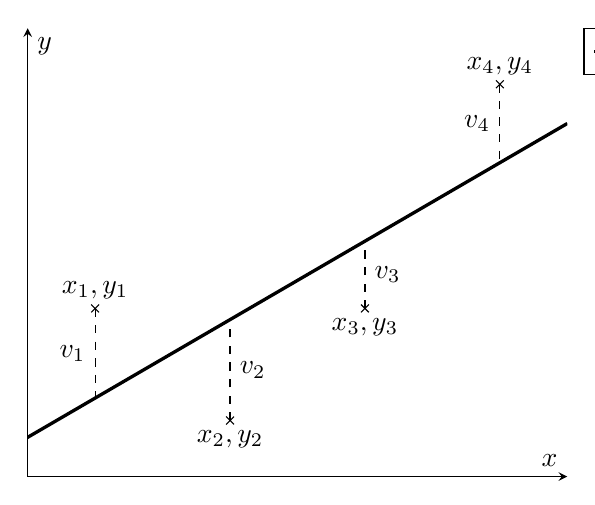
\begin{tikzpicture}[trim axis left, trim axis right]
        \begin{axis}[
            xlabel = {$x$},
            ylabel = {$y$},
            xtick = \empty,
            ytick = \empty,
            ylabel style={rotate=-90},
            xmin = 0.5,
            xmax = 4.5,
            ymin = 0,
            ymax = 8,
            domain = 0:4.5,
            samples = 101,
            axis y line=middle,
            axis x line=middle,
            legend cell align={left},
            legend pos=outer north east,
        ]

        \addplot[very thick] {1.4 * x};
        \addlegendentry{$y = a + bx$};

        \addplot [
            scatter,
            only marks,
            point meta=explicit symbolic,
            scatter/classes={
                a={mark=x}
            },
        ] table [meta=label] {
            x    y   label
            1    3   a
            2    1   a
            3    3   a
            4    7   a
        };
        
        \draw[dashed] (1, 3) -- (1, 1.4);
        \draw[dashed] (2, 1) -- (2, 2.8);
        \draw[dashed] (3, 3) -- (3, 4.2);
        \draw[dashed] (4, 7) -- (4, 5.6);

        \node[anchor=south] at (1, 3) {$\bp{x_1, y_1}$};
        \node[anchor=north] at (2, 1) {$\bp{x_2, y_2}$};
        \node[anchor=north] at (3, 3) {$\bp{x_3, y_3}$};
        \node[anchor=south] at (4, 7) {$\bp{x_4, y_4}$};

        \node[anchor=east] at (1, 2.2) {$v_1$};
        \node[anchor=west] at (2, 1.9) {$v_2$};
        \node[anchor=west] at (3, 3.6) {$v_3$};
        \node[anchor=east] at (4, 6.3) {$v_4$};
        \end{axis}
    \end{tikzpicture}
    \caption{The vertical residuals as vertical distances between actual and observed values.}
\end{figure}

\begin{definition}
    The \vocab{least-squares regression line of $y$ on $x$} is obtained by finding the values of $a$ and $b$ in $y = a + bx$ that minimizes the sum of the squares of the vertical residuals, $S$: \[S = \sum_{i = 1}^n v_i^2 = \sum_{i = 1}^n \bs{y_i - \bp{a + bx_i}}^2.\]
\end{definition}

The values of $a$ and $b$ that minimize $S$ is called the \vocab{least-squares estimates} of $a$ and $b$. $b$ is also sometimes called the \vocab{regression coefficient}.

The following result can be shown using functions of two variables (see~\nameref{S::Assignment-B11} Problem 3):

\begin{proposition}
    The regression line of $y$ on $x$ is given by $y - \ol{y} = b \bp{x - \ol{x}}$ where \[b = \frac{\sum \bp{x-\ol{x}} \bp{y - \ol{y}}}{\sum \bp{x-\ol{x}}^2} = \frac{\sum xy - n \bp{\ol{x}}\bp{\ol{y}}}{\sum x^2 - n \bp{\ol{x}}^2}.\]
\end{proposition}

Observe that the regression line of $y$ on $x$ passes through the \vocab{mean point} $\bp{\ol{x}, \ol{y}}$.

\subsection{Regression Line of $x$ on $y$}

The regression line of $x$ on $y$ is similar. In this case, however, we are concerned with \emph{horizontal} deviations instead.

\begin{definition}
    The \vocab{horizontal residual}, denoted $h_i$, is the deviation between the actual and predicted $x$-values. \[h_i = y_i - \bp{c + d x_i}\] for some constants $c$ and $d$.
\end{definition}

Analogous to $v_i$, we can think of a horizontal residual as the (signed) \emph{horizontal} distance between an observed data point $(x_i, y_i)$ and the line $x = c + dy$.

\begin{figure}[H]\tikzsetnextfilename{486}
    \centering
    \begin{tikzpicture}[trim axis left, trim axis right]
        \begin{axis}[
            xlabel = {$x$},
            ylabel = {$y$},
            xtick = \empty,
            ytick = \empty,
            ylabel style={rotate=-90},
            xmin = 0.5,
            xmax = 5.5,
            ymin = 0,
            ymax = 8,
            domain = 0:5.5,
            samples = 101,
            axis y line=middle,
            axis x line=middle,
            legend cell align={left},
            legend pos=outer north east,
        ]

        \addplot[very thick] {x * 2.714 - 3.2857};
        \addlegendentry{$x = c + dy$};

        \addplot [
            scatter,
            only marks,
            point meta=explicit symbolic,
            scatter/classes={
                a={mark=x}
            },
        ] table [meta=label] {
            x    y    label
            1    3    a
            2    1    a
            3    3    a
            4    7    a
        };

        \coordinate[label=above:$\bp{x_1, y_1}$] (P1) at (1, 3);
        \coordinate[label=right:$\bp{x_2, y_2}$] (P2) at (2, 1);
        \coordinate[label=right:$\bp{x_3, y_3}$] (P3) at (3, 3);
        \coordinate[label=right:$\bp{x_4, y_4}$] (P4) at (4, 7);
        \coordinate (Y1) at (1.57911, 1);
        \coordinate (Y3) at (2.31603, 3);
        \coordinate (Y7) at (3.78987, 7);

        \draw[dashed] (Y3) -- (P1);
        \draw[dashed] (Y1) -- (P2);
        \draw[dashed] (Y3) -- (P3);
        \draw[dashed] (Y7) -- (P4);

        \node[anchor=north] at ($(Y3)!0.5!(P1)$) {$h_1$};
        \node[anchor=north] at ($(Y1)!0.5!(P2)$) {$h_2$};
        \node[anchor=north] at ($(Y3)!0.5!(P3)$) {$h_3$};
        \node[anchor=north] at ($(Y7)!0.5!(P4)$) {$h_4$};
        \end{axis}
    \end{tikzpicture}
    \caption{The horizontal residuals as horizontal distances between actual and observed values.}
\end{figure}

\begin{definition}
    The \vocab{least-squares regression line of $x$ on $y$} is obtained by finding the values of $c$ and $d$ in $x = c + dy$ that minimizes the sum of the squares of the horizontal residuals, $S$: \[S = \sum_{i = 1}^n h_i^2 = \sum_{i = 1}^n \bs{x_i - \bp{c + d y_i}}^2.\]
\end{definition}

\begin{problem}
    The regression line of $x$ on $y$ is given by $x - \ol{x} = d\bp{y - \ol{y}}$, where \[d = \frac{\sum \bp{x - \ol{x}} \bp{y - \ol{y}}}{\sum \bp{y - \ol{y}}^2} = \frac{\sum xy - n \bp{\ol{x}}\bp{\ol{y}}}{\sum y^2 - n \bp{\ol{y}}^2}.\]
\end{problem}

As in the $y$ on $x$ case, we call $d$ the regression coefficient. Note that $1/d$, and not $d$, is the gradient of the regression line. Observe that the regression line of $x$ on $y$ also passes through the mean point $\bp{\ol{x}, \ol{y}}$.

\subsection{Determining Which Regression to Use}

If there is an independent variable $x$, we use the regression line $y$ on $x$ regardless of whether we are predicting or estimating $y$ or $x$, and vice versa when $y$ is the independent variable.

However, if there is no clear dependent-independent relationship, we determine the independent variable based on the given value. For example, if we are given the value of $x$, we use the regression line $y$ on $x$.

\subsection{Interpolation and Extrapolation}

\begin{definition}
    An estimate is said to be an \vocab{interpolation} if it is within the given range of values of data. Else, it is an \vocab{extrapolation}.
\end{definition}

Extrapolation of the sample should be used with caution as the relationship between $x$ and $y$ may not be linear beyond a certain point.

\subsection{Reliability of an Estimate}

There are three criteria we typically use when commenting on the reliability of an estimate:
\begin{itemize}
    \item Appropriateness of the regression line used -- The correct regression line should be used for the estimate to be reliable.
    \item Strength of linear correlation -- $\abs{r}$ should be close to 1 for the estimate to be reliable.
    \item Interpolation or extrapolation -- Interpolation is likely to give a more reliable estimate than extrapolation.
\end{itemize}

For an estimate to be reliable, all three criteria should be satisfied. If at least one of the criteria is not satisfied, we deem the estimate to be unreliable.

\section{Transformations to Linearize Bivariate Data}

The relationship between two variables involved, $x$ and $y$, may not always be linear. Thus, it would be inappropriate to use the regression lines relating to $x$ and $y$ to make estimations. However, non-linear relationships can be transformed into a linear form by a process usually called \vocab{transformation to linearity}. The table below shows some examples:

\begin{table}[H]
    \centering
    \begin{tabular}{|c|c|c|}
        \hline
        \textbf{Original Equations} & \textbf{Transformed Equations} & \textbf{Linearly-related Expressions} \\ \hline
        $y = a + bx^2$ & - & $y$ vs $x^2$ \\ \hline
        $y = ab^x$ & $\ln y = \ln a + x \ln b$ & $\ln y$ vs $x$ \\ \hline
        $y = ax^b$ & $\ln y = \ln a + b \ln x$ & $\ln y$ vs $\ln x$ \\ \hline
    \end{tabular}
\end{table}

Sometimes, we are given a scatter diagram and are tasked with comparing two or more proposed models and determine which model is a better fit. In such a scenario, we simply state which equation fits the shape of the scatter plot better. If there is more than one possibility, we can compute the product moment correlation coefficient for each model and ``break the tie'' by choosing the model with $\abs{r}$ closest to 1.

\section{Bonus: A Probabilistic Approach to Linear Regression}

In an ideal world, our variables will be exactly related by the model $y = a + bx$. However, in the real world, whenever we observe a data point, our readings will contain some error $\ep$, so our observations are actually modelled by $y = a + bx + \ep$. In real life, these errors are caused by thousands of different factors. We can hence think of $\ep$ as the sum of many independent random variables. But by the Central Limit Theorem, it follows that $\ep$ is distributed normally, so \[\ep \sim \Normal{0}{\s^2}.\]

Suppose now that we obtain an observation, $\bp{x_i, y_i}$. Since $\ep_i = y_i - \bp{a + bx_i}$, the probability of observing this data point is given by \[\P{(x_i, y_i)} = \P{\ep = \ep_i} = \P{\ep = y_i - \bp{a + bx_i}} = \frac1{\sqrt{2\pi} \s} \exp{-\frac{\bp{y_i - \bp{a + bx_i}}^2}{2\s^2}}.\] If we make $n$ \emph{independent} observations, then the overall probability of observing all $n$ data points is simply the product of each individual probability: \[\P{\text{data}} = \prod_{i = 1}^n \frac1{\sqrt{2\pi} \s} \exp{-\frac{\bp{y_i - \bp{a + bx_i}}^2}{2\s^2}}.\]

It is now natural to define the ``best'' model ($y = a + bx$) as the one that maximizes the probability of observing our data. That is, we wish to find $a$ and $b$ that maximizes \[\prod_{i = 1}^n \frac1{\sqrt{2\pi} \s} \exp{-\frac{\bp{y_i - \bp{a + bx_i}}^2}{2\s^2}}.\] Since the logarithm is monotonic, we can convert our objective function from a product into a sum: \[\argmax_{a, b} \ln \prod_{i = 1}^n \frac1{\sqrt{2\pi} \s} \exp{-\frac{\bp{y_i - \bp{a + bx_i}}^2}{2\s^2}} = \argmax_{a, b} \sum_{i = 1}^n \bp{-\frac{\bp{y_i - \bp{a + bx_i}}^2}{2\s^2}},\] where we ignored the constant terms contributed by $1/\sqrt{2\pi} \s$ since they do not affect the location of the maxima. We can further ignore the $1/\s^2$ term since it is a constant factor. Lastly, flipping the sign changes our objective into a minimization problem, so we get \[\argmin_{a, b} \sum_{i = 1}^n \bp{y_i - \bp{a + b x_i}}^2.\] But this is exactly the objective of the least-squares regression line of $x$ on $y$ we introduced earlier!

\section{Bonus: $r$ and Vectors}

Suppose we have two sets of data, say $x_1, \dots, x_n$ and $y_1, \dots, y_n$. Let $\ol{x}$ and $\ol{y}$ denote their respective means. Recall that the product moment correlation coefficient $r$ between these two samples is given by \[r = \frac{\sum \bp{x - \ol{x}} \bp{y - \ol{y}}}{\sqrt{\sum \bp{x - \ol{x}}^2 \sum \bp{y - \ol{y}}^2}}.\] Observe that the definition of $r$ resembles the definition of the cosine of an angle between two vectors! Indeed, if we define \[\vec x = \cveciii{x_1 - \ol{x}}{\vdots}{x_n - \ol{x}} \quad \tand \quad \vec y = \cveciii{y_1 - \ol{y}}{\vdots}{y_n - \ol{y}},\] then we can simply express $r$ as \[r = \frac{\vec x \dotp \vec y}{\abs{\vec x}^2 \abs{\vec y}^2} = \cos \t,\] where $\t$ is the angle between the two vectors $\vec x$ and $\vec y$.\footnote{We can think of these two vectors as the ``deviation'' between the sample data and their respectively means. Indeed, it is not too hard to see that the sample variances are given by $s_X^2 = \frac1{n-1} \abs{\vec x}^2$ and $s_Y^2 = \frac1{n-1} \abs{\vec y}^2$. The scaled dot product $\frac1{n-1} \bp{\vec x \dotp \vec y}$ also has a special name, called the ``sample covariance'', typically denoted $s_{XY}^2$, so the product moment correlation coefficient can be expressed more succinctly as \[r = \frac{s_{XY}^2}{s_X s_Y}.\]} Similarly, we can rewrite the regression coefficients $b$ and $d$ vectorially: \[b = \frac{\vec x \dotp \vec y}{\abs{\vec x}^2} \quad \tand \quad d = \frac{\vec x \dotp \vec y}{\abs{\vec y}^2}.\] If we manipulate the above two expressions, we see that \[b = \frac{\vec{\hat x} \dotp \vec y}{\abs{\vec x}} \quad \tand \quad d = \frac{\vec x \dotp \vec{\hat{y}}}{\abs{\vec y}}.\] Now observe that the numerator of $b$ is exactly the length of projection of $\vec y$ onto $\vec x$. Similarly, the numerator of $d$ is exactly the length of projection of $\vec x$ on $\vec y$.

That is to say, $b$ measures the ratio between the vector projection of $\vec y$ onto $\vec x$, and similarly for $d$: \[b = \frac{\text{length of projection of $\vec y$ onto $\vec x$}}{\text{length of $\vec x$}} \quad \tand \quad d = \frac{\text{length of projection of $\vec x$ onto $\vec y$}}{\text{length of $\vec y$}}.\] This aligns with our intuition of $b$ and $d$: If the two samples share a strong linear correlation, we would expect the regression lines of $y$ on $x$ and $x$ on $y$ to be roughly the same. Indeed, $\vec x$ and $\vec y$ are roughly multiples of each other, say $\vec x \approx \l \vec y$ for some $\l$, so \[b \approx \frac{\abs{\l \vec y}}{\abs{\vec y}} = \abs{\l} \quad \tand \quad d \approx \frac{\abs{\vec x}}{\abs{\l \vec x}} = \frac1{\abs{\l}} \implies b \approx \frac1{d}.\] But $b$ and $1/d$ represent the gradients of the regression lines of $y$ on $x$ and of $x$ on $y$ respectively, so the two lines have roughly equivalent gradients, i.e. the two lines are roughly the same.